% Example LaTeX document for GP111 - note % sign indicates a comment
\documentclass{article}

\usepackage{graphicx}
\usepackage{titlesec}
\usepackage{titling}

\graphicspath{ {images/} }

\titleformat{\section}
{\normalfont\normalsize\bfseries}{\thesection}{1em}{}

\posttitle{\par\end{center}}
\setlength{\droptitle}{-20pt}

% Default margins are too wide all the way around. I reset them here
\setlength{\topmargin}{-.5in}
\setlength{\textheight}{9in}
\setlength{\oddsidemargin}{.125in}
\setlength{\textwidth}{6.25in}

\begin{document}
\title{Multi-Threaded Matrix Multiply}
\author{Jesse Bannon\\
University of Washington, Tacoma}
\renewcommand{\today}{July 2, 2017}
\maketitle

In this paper, I outline the performance characteristics between three implementations of dense matrix-matrix multiply: single-threaded, multi-threaded, and multi-threaded Strassen algorithm. Each implementation stores matrices row-major in memory and uses double-precision floating points. These metrics were gathered using an Intel i7 5820K CPU, which includes six cores and twelve threads using Intel's Hyper-Threading Technology.

\paragraph{Single-Threaded}
One core performs a matrix-matrix multiply $C = AB$ using a trivial triple-nested for-loop.

\paragraph{Multi-Threaded}
Each thread $t_{i}$ performs a subset of the matrix-matrix multiply $C_{i} = AB_{i}$, where $B$ is partitioned by sequential columns $B_{i} = \lbrace b_{j}, b_{j+1}, \dots, b_{j+n} \rbrace$ evenly amongst all $t_{i}$. In the case that $B$'s columns are greater than the number of threads, we assign a single column to a subset of threads and leave the remaining idle.

\paragraph{Strassen Algorithm}
Each operation (dense matrix-matrix add, subtract, multiply) of the Strassen algorithm is multi-threaded amongst all threads. Every matrix-matrix multiply recursively calls Strassen algorithm, inconsequently performing a depth-first traversal in the recursion. After the split input matrix size reaches a certain threashold, the multi-threaded implementation is used.

\begin{figure}[h]      
	\centering 
    \fbox{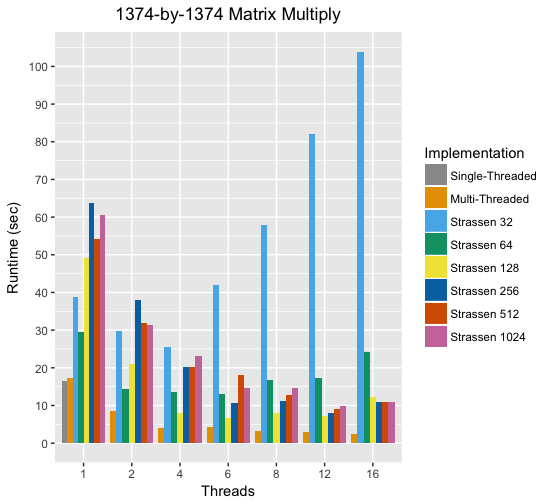
\includegraphics[width=.3\textwidth]{1374-multiply.png}}   
    \hspace{10px}
    \fbox{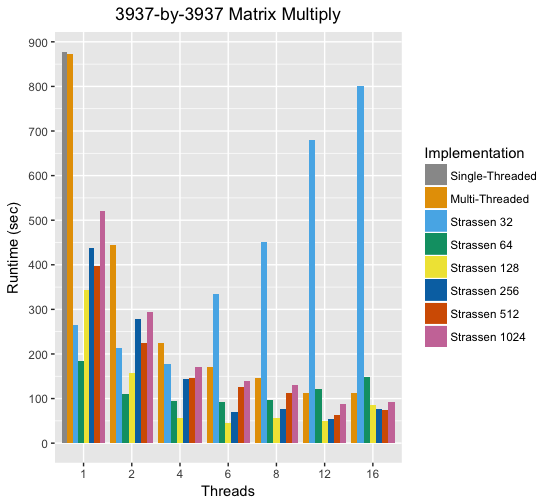
\includegraphics[width=.3\textwidth]{3937-multiply.png}}
    \hspace{10px}
    \caption{Elapsed time to perform dense matrix-matrix multiply}
    \label{materialflowChart}
\end{figure}

When multiplying a 1374-by-1374 matrix with itself, the 16-thread multi-threaded multiply performed the best with a $2.46$ second runtime. Each thread was responsible to multiply the matrix with its (approximately) 1375-by-85 subset.  The performance comes from the memory lookups on $B$ when multiply its columns. The Strassen algorithm, in this case, over-parallelized the problem size.
\linebreak

The 3937-by-3937 matrix performs best using the 6-thread Strassen algorithm, with a 128-size stopping condition for dense matrix-matrix multiplies, in $45.11$ seconds. The second best metric has the same configuration except it uses 12 threads. In this case, hyper-threading decreases performance. The problem size in this case is large enough to where the Strassen algorithm does not over-parallelize, which takes advantage of its lower complexity of $\mathcal{O}(n^{log_{2}{7}})$ compared to the traditional matrix-multiply complexity of $\mathcal{O}(n^3)$.

\end{document}